%%   This file is part of the APS files in the REVTeX 4 distribution.
%%   Version 4.0 of REVTeX, August 2001
%%
%%
%%   Copyright (c) 2001 The American Physical Society.
%%
%%   See the REVTeX 4 README file for restrictions and more information.
%%
%
% This is a template for producing manuscripts for use with REVTEX 4.0
% Copy this file to another name and then work on that file.
% That way, you always have this original template file to use.
%
% Group addresses by affiliation; use superscriptaddress for long
% author lists, or if there are many overlapping affiliations.
% For Phys. Rev. appearance, change preprint to twocolumn.
% Choose pra, prb, prc, prd, pre, prl, prstab, or rmp for journal
%  Add 'draft' option to mark overfull boxes with black boxes
%  Add 'showpacs' option to make PACS codes appear

% Edited by Camilla Harris Jan 2015
% For use by Camilla Harris, Akshat Mahajan
% in creating Lab Reports for 180c at UCLA
% this file and auxiliary files were retrieved from
% http://www-d0.fnal.gov/Run2Physics/WWW/templates/
% on Jan 19 2015

\documentclass[aps,prl,nofootinbib,twocolumn,superscriptaddress,groupedaddress]{revtex4}  % for review and submission
%\documentclass[aps,preprint,superscriptaddress,groupedaddress]{revtex4}  % for double-spaced preprint
% CAMILLA: I removed the PACS functionality
\usepackage{graphicx}  % needed for figures
	%if using postscript files compile with XeLaTex
\usepackage{dcolumn}   % needed for some tables
\usepackage{bm}        % for math
\usepackage{amssymb}   % for math
\usepackage[export]{adjustbox}
\usepackage{array}
\newcolumntype{P}[1]{>{\centering\arraybackslash}p{#1}}

% avoids incorrect hyphenation, added Nov/08 by SSR
\hyphenation{ALPGEN}
\hyphenation{EVTGEN}
\hyphenation{PYTHIA}

\begin{document}
\title{Physics 180C Lab Report 1: Superconductivity}
\input author_list.tex        % includes institutions and visitors
\date{\today}

\begin{abstract}
The distribution of critical fields with respect to temperature $H_{c}(T)$ were measured for the superconducting metals indium, lead and tin between 0 to 7 K, and compared to a theoretical fit of the form $H_{c}(T) = H_{c}(0)\cdot(1 - (T/T_{c})^{2})$. It was found that, while our observations obeyed a negative quadratic distribution commensurate with our theoretical fit ($r^{2} \geq$ 0.99 for all samples), constant offsets were noted that prevented an exact fit to each data point. The percentage error in our estimates, obtained by comparing known $H_{c}(0)$ values with our extrapolated values, are (for indium) 8.56\%, (for tin) -1.61\%, and (for lead) 12.43\%. We analyse our results in this paper. 
\end{abstract}

\maketitle

\section{Background Information}

Superconducting metals are known to undergo a transition into the superconducting state at a characteristic temperature (called the \textsl{critical temperature}, denoted by $T_{c}$), where they demonstrate an abrupt drop in magnetic susceptibility (the Meissner effect) and consequently inductance. Exposure to a sufficient amount of magnetic field below the critical temperature, however, is capable of destroying this superconducting state. We call the minimum value of the field needed to force the superconductor back into a normal state the \textsl{critical field}, and denote it by $H_{c}$. Theoretical examinations of this phenomenon have obtained an approximate relationship between the temperature $T$ of the sample and the critical field at that temperature\cite{kittel}:
\begin{equation}
H_{c}(T) = H_{c}(0) \cdot \left[ 1 - \left(\frac{T}{T_{c}}\right)^{2}\right]
\end{equation}
 
We attempted to experimentally document this behaviour for three superconducting elements, namely indium, tin and lead. Samples were initially kept in a low vacuum chamber and cooled down to 2 K (well below each metal's critical temperature) in a liquid helium bath. The sample's inductance $L$ was used as a proxy for the superconducting state, and was indirectly measured through an oscillatory circuit setup with the sample acting as the inductor. The frequency $\omega$ of the oscillatory circuit exhibited the following approximate relationship with the inductance:
$$ \omega = \frac{1}{\sqrt{LC}} \propto \frac{1}{\sqrt{L}}$$ where $C$ was the capacitance of the circuit. As the sample transitioned from the superconducting state to the normal state, the inductance would suddenly and sharply increase, leading to a simultaneous decrease in frequency. This behaviour allowed us to use the frequency as an indicator of the inductance value.

At a particular temperature, the sample would be exposed to successively increasing external magnetic fields until an abrupt drop in frequency was recorded, indicating a transition from superconducting to normal state. We measured all three samples at the same temperature, switching our frequency monitor from one sample to another after every measurement. We identified the critical field as the field following which the $\omega$ vs. $H$ curve exhibited the most negative slope; a MATLAB script was used to identify this point post-experiment. The temperatures we investigated were 2.09 K, 2.17 K, 2.23 K, 2.33 K, 2.49 K, 2.716 K, 3.01 K, 3.6 K, 4.06 K, 5 K, 5.99 K, 6.58 K, and 7.07 K. We did not investigate samples at temperatures above their critical temperature. Finally, once the corresponding critical field for each temperature had been obtained, the collected values were plotted against temperature for the sample, and fitted against the  relationship given by (1). 

It was found that using known values of $H_{c}(0)$ and $T_{c}$ for each sample was unable to provide an exact fit to our observations, with significant offsets from the fit noted for each data point; however, a strong negative quadratic relationship with temperature, in line with (1), was documented. The degree-of-freedom corrected correlation coefficient for our data with the fit prescribed by (1) was in excess of 0.99, indicating a robust fit, for all samples. We experimented with allowing either $H_{c}(0)$ or both $H_{c}(0)$ and $T_{c}$ to vary to test different models of error in our experiment, and found significant evidence (via the statistical F test) for temperature differentials between our temperature measurement apparatus and our tin sample, as well as partial oxidation for lead, as the leading sources of error. Extrapolations for $H_{c}(0)$ were obtained from those error models that passed the F test and could be said to `better' fit the data than competing models.

\section{Results}

Here we include graphs and tables of our final data. Raw data is available on request. Pink errorbars indicate the negative slopes following these points in the raw data was less than three standard deviations from the mean of the negative slopes, from which we have estimated the error in picking the point of most negative slope. Most finally chosen points were above the three standard deviations mark, and thus have no associated errorbars. We explain our procedure in detail in our next section.

\begin{figure}
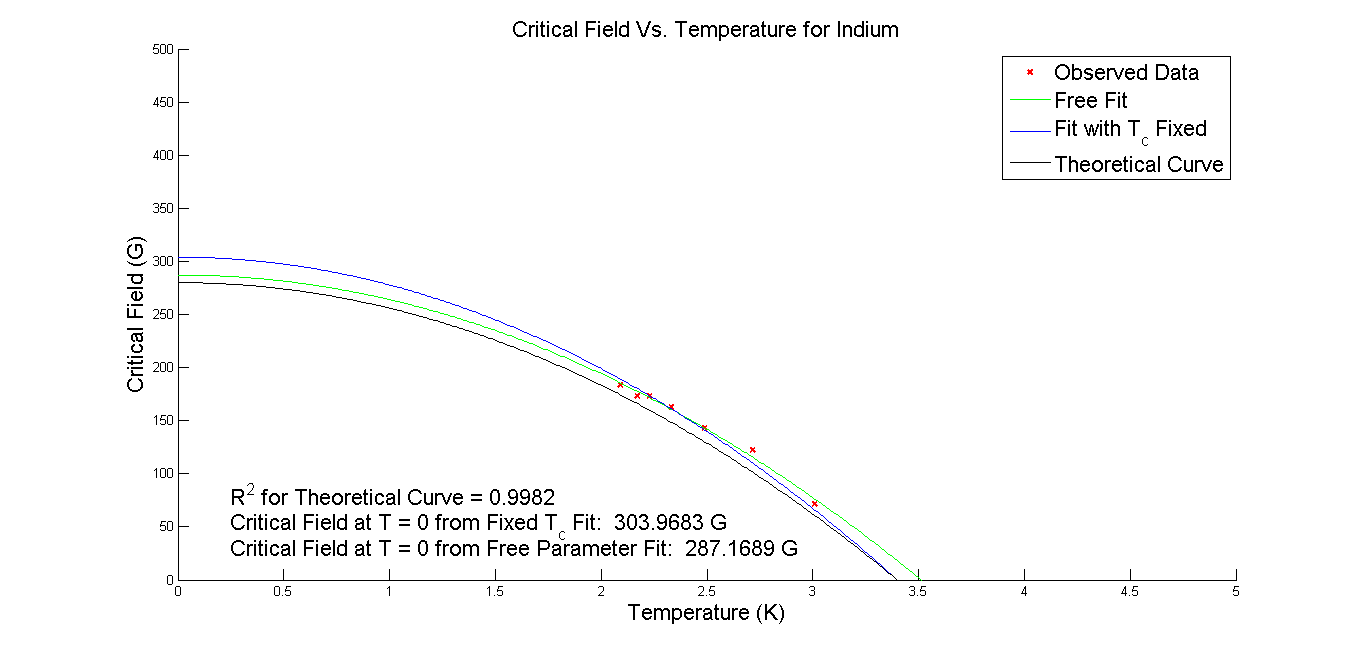
\includegraphics[width = 0.55\textwidth, right, height = 5.4cm]{../Analysis/IndiumFieldVsTempPicture.png}
\caption{A line plot detailing best fits for indium} 
\end{figure}

\begin{figure}
\centering
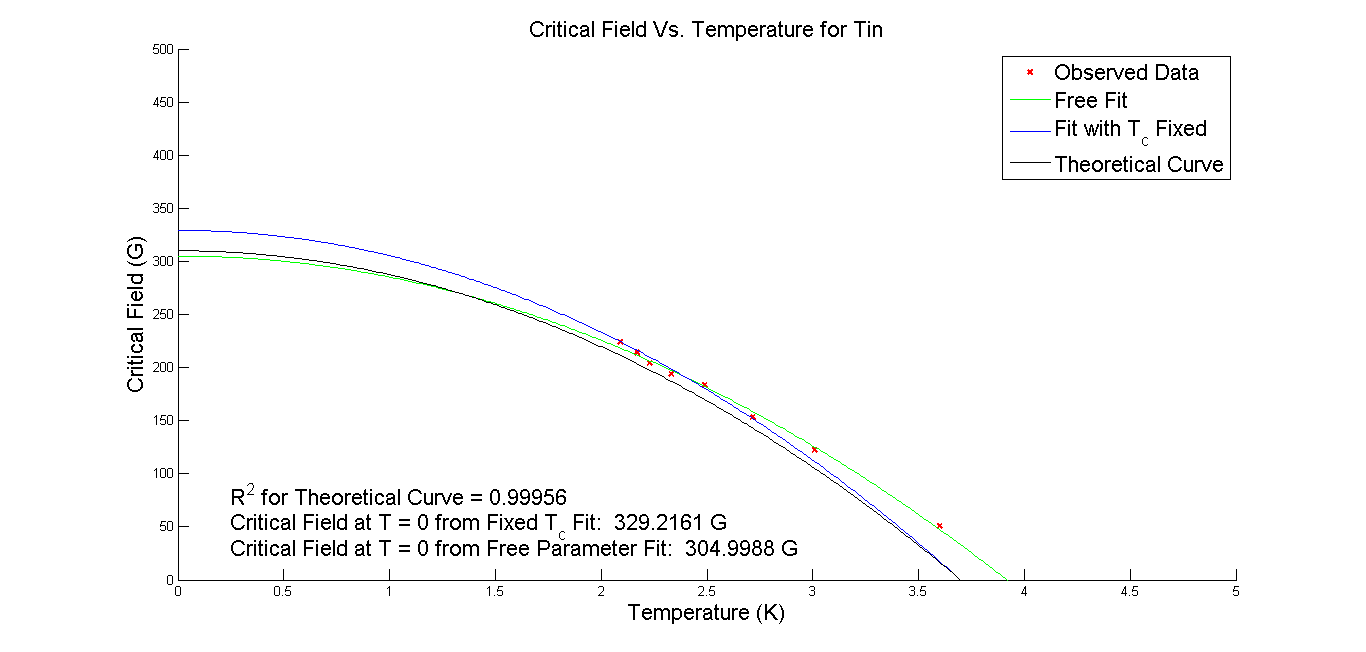
\includegraphics[width = 0.55\textwidth, right, height = 5.4cm]{../Analysis/TinFieldVsTempPicture.png}
\caption{A line plot detailing best fits for tin} 
\end{figure}

\begin{figure}
\centering
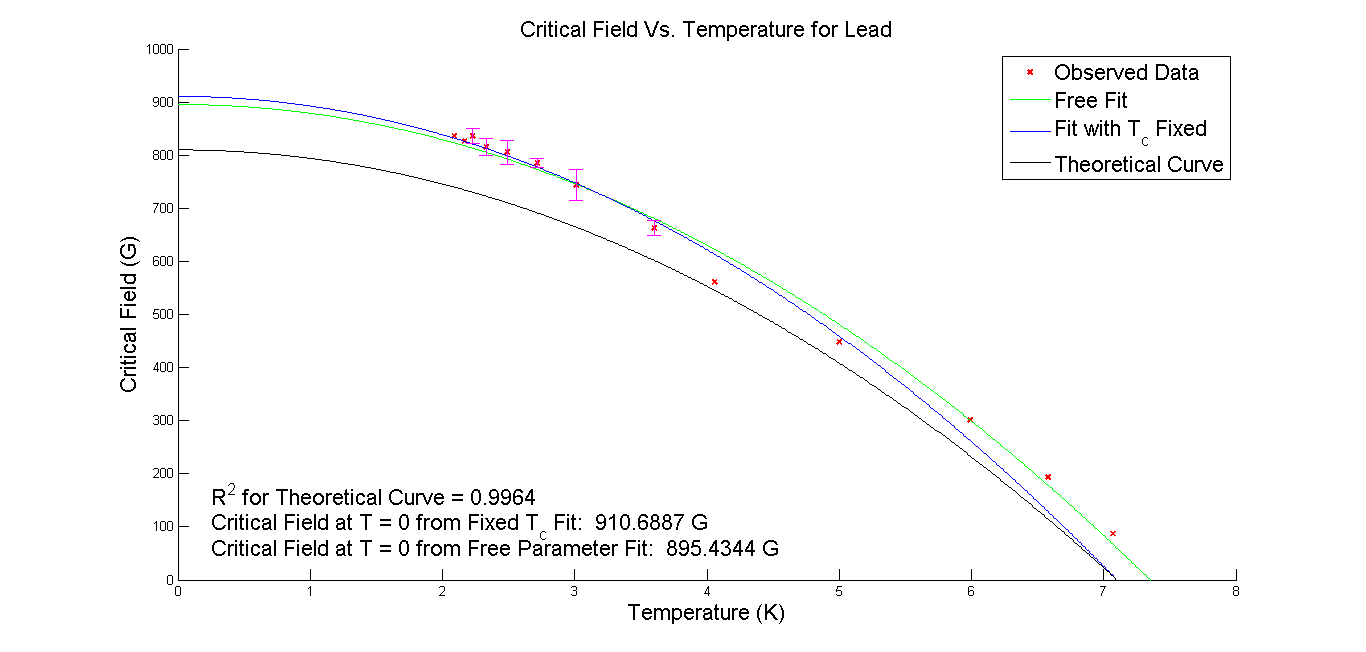
\includegraphics[width = 0.55\textwidth, right, height = 5.4cm]{../Analysis/LeadFieldVsTempPicture.png}
\caption{A line plot detailing best fits for lead} 
\end{figure}

\begin{table}
\caption{\label{tab:table1} A table listing the value of all nonzero symmetric errorbars (displayed in pink in Figs. 1, 2, and 3) divided in half, and the corresponding field values for which they occured. All units in Gauss unless otherwise stated.}
\begin{ruledtabular}
\begin{tabular}{lcccP{0.15\textwidth}}
Sample&Error Value& Field& T (K)& Percent Error(\%)\\
\hline
Lead & 14.41 & 835.90& 2.23&  1.72\\
Lead & 16.27 & 815.52 & 2.33 & 2.00\\
Lead & 22.94 & 805.32 & 2.49 & 2.85\\
Lead & 8.70 & 784.93 & 2.71 & 1.11\\
Lead & 28.83 & 744.16 & 3.01 & 3.87\\
Lead & 14.41 & 662.61 & 3.6 & 2.18\\
\end{tabular}
\end{ruledtabular}
\end{table}

\begin{table}
\caption{A table listing the results of our F-test for the `free-fit' model and model with $T_{c}$ fixed (`fixed-fit'). $\alpha$ denotes our level of significance.}
\begin{ruledtabular}
\begin{tabular}{lP{0.15\textwidth}ccP{0.15\textwidth}}
Sample& F-test Value & $\alpha$ & P  $< \alpha$& Accept Free-Fit? \\
\hline
Indium  & 13.69\% & 5\% & No & No\\
Tin & 0.41\% & 5\% & Yes & Yes \\
Lead & 10.11\% & 5\% & No & No \\

\end{tabular}
\end{ruledtabular}
\end{table}

\section{\label{sec:level2}Analysis and Related Discussion}
From the graphs preceding this section, it is clear that the data points are offset from our fit, but otherwise obey a negative quadratic relationship with temperature in line with (1). Here, we investigate several sources of error that may have led to this result, and assess their contribution.  

We identified the following random errors: significant trends and fluctuations in the frequency, occasionally above the magnitude of the drop associated with the transition to the normal state; and temperature differentials between the temperature probe and the sample. We identified the following possible sources of error: inconsistent choice of field ranges and step delay times; consistently picking the point preceding the most negative slope as our critical field for that temperature; the order of measurement of samples, wherein we would cycle through the samples and then use the last sample at one temperature as the first sample to be measured at a new temperature, leading to the frequency monitor to be fixed at a sample longer than the other ones. We identified the following systematic errors: the use of a partly oxidized lead sample; and no repeated measurements for $\omega$ vs. $H$ at a particular temperature for a particular sample.

We first estimated the contribution from picking the point preceding the most negative slope as our critical field. Our choice of using this as our indicator of the critical field stems from the expectation that the negative slope due to transition is the most dominant signal in the data. Were the negative slopes entirely due to random errors, it is expected that the distribution of negative slopes should also be random; a negative slope due to actual transition from the superconducting to normal state would then be well above the range of the randomly distributed negative slopes if we knew the random errors were in fact \textit{small} compared to the actual transition slope. However, our measurement was not ideal: random fluctuations in inductance led to trends in the frequency below and beyond the supposed critical field level, while it was expected for the $\omega$ vs. $H$ field to resemble more of a downward step function. An error might arise if the minimum negative slope was comparable with other negative slopes due entirely to random fluctuations - there is always the possibility that our chosen slope might itself have been due to a random error and not, in fact, due to transition. We cannot directly calculate the effect of the random errors from our experimental setup, however, as there are too many experimental factors to assess. To work around this, we first model the distribution of slopes as a normal (Gaussian) distribution, and then attempt to calculate the $z$-score\footnote{The z-score of a value is the difference between the value and the standard deviation $\sigma$ divided by the mean $\mu$ i.e. $Z(x) = \frac{x - \sigma}{\mu}$} of our chosen most negative slope. Our $z$-score calculation did not eventually factor into our error analysis; we mention it here to offer some illustration of the low chance of reproduction from random sources. From elementary statistics, points with a $z$-score $ \geq 3$ have less than 1\% chance of arising randomly. 

Most of our chosen slopes have $z$-scores greater than 3. However, this is not true for all slopes. Regardless of $z$-score, we attempted to find recorded slope values neighbouring (i.e. within the range $x \pm \sigma$ for standard deviation $\sigma$ of all slopes) from our chosen most negative value $x$. We would then find the fields corresponding to these neighbouring values, and express our error as the standard deviation of these fields. Where no negative slopes within one standard deviation from our chosen negative slope exist (in other words, within the conventional range of error), there the error is taken to be 0. Those are the points that appear with no errorbars in Figures (1), (2) and (3). We chose standard deviation as our key metric as we assume we had equal probability of choosing any of the fields that lie in the neighbourhood of our chosen most negative slope. Our errors are very small: the largest error encountered is approximately 28 Gauss for lead sample at 3.0 K, indicating only a 4\% possible change in critical field value at that temperature for that sample. We include a list of all error values and the corresponding field values and temperatures for lead, the only sample to demonstrate error, in Table 1. 

It is worth noting that this method of estimating error in our measurements allows us to address errors from several other possible sources, and conclude that they are negligible. The key value returned in each run is the critical field, by virtue of using the most negative slope as our indicator. By demonstrating that, in most cases, the chosen negative slope has less than 1\% chance of occurring randomly, we can argue that random errors had a minimal effect on our choice. By further demonstrating that, for all but a select few points, no slope of comparable magnitude exists within one standard deviation from the chosen negative slope, we can successfully argue that effects from inconsistent sources of error (i.e. those that only affect some $\omega$ vs. H graphs such as order of transition; inconsistent step sizes) do not have a statistically significant effect on the distribution of slopes for the samples they did affect. More testing may be needed to verify the claim that these potential sources had minimal impact on our samples, but as a first-order result, errors due to these known inconsistent potential sources do not appear to have propagated to our choice of critical field for any temperature. 

Now we consider sources of error that may have been applied consistently for every measurement for a sample. We investigated the contribution from temperature differentials between the sample and the temperature probe. Owing to the fact that no measurements were repeated for any temperature or sample, we were unable to test this hypothesis for each temperature (intra-temperature), and were forced instead to attempt to test it over the entire temperature range (inter-temperature). To do this, we reasoned that roughly constant temperature differentials should cause an offset, either to the left or right, from the actual distribution, and that, from Eq. (1), this should translate to a shift in apparent critical temperature. We then constructed two models: a `free-parameter' model of the form of (1) where $H_{c}(0)$ and $T_{c}$ were allowed to vary; and a `fixed-fit' model where only $H_{c}(0)$ was allowed to vary. Both the final forms of the `fixed-fit' and `free-fit' model were obtained using the MATLAB \texttt{nlinfit} function, which allows for nonlinear regression modelling. We also defined the theoretical curve as given by (1) for known $H_{c}(0)$ and $T_{c}$.  All three curves are modeled, alongside the data, in each figure in the Result section.

To compare which one of these two fit models was statistically `better', we performed a statistical F test, which is used to compare nested models (models that differ by only one additional parameter)\cite{ftest}. The F test computes the probability that the explained improvement in fit from the `free-fit' model over the `fixed-fit' model can be attributed to the effect from the addition of an extra parameter, instead of due to what the extra parameter represents. Our level of significance - the probability below which we were willing to accept that the inclusion of an additional parameter is due to the nature of the parameter rather than simply its inclusion - was 5\%; probability values below this indicate that the `free-fit' model better explains the data observations. The results of our F test for each sample are displayed in Table 2, alongside whether we chose to accept that temperature differentials (represented by the `free-fit' model) played a significant role. Not choosing to accept the `free-fit' model does not mean a rejection of it, merely the conclusion that there is insufficient statistical evidence to argue that the `fixed-fit' model be rejected\cite{ftest}.

Finally, we note that significant oxidation is known to have taken place for the lead sample. Estimating the effect due to this is difficult, as the impurity concentration nor the type of particular oxidation (i.e. whether PbO or PbO$_{2}$) of the sample was unknown at the time of experiment. According to Anderson theory (appropriate for Type I superconductors) \cite{impuresuper}, there should not be a significant effect from impurities - however, this behaviour does not appear to be demonstrated in our samples. We are unable to provide an estimate of its effect at this time (although we do note it is clearly significant from the discrepancy between our data and underlying theory).

From the preceding discussion, we are finally at a point where we can estimate $H_{c}(T \rightarrow 0)$ meaningfully from $T_{c}$ values. From the the `fixed-fit model', we obtain values of 303.96 G for indium (off by 8.56\%; accepted value is 280 G), 329.21 G for tin (off by 10.61\%; accepted value is 310 G) and 910.68 G for lead (off by 12.43\%). However, we found compelling evidence to favour the `free-fit' model over the `fixed-fit' values for tin. For tin, the obtained value from the `free-fit' model is 304.99 G (off by -1.61\%). The final values we report are 303.96 G for indium, 304.99 G for tin, and 910.68 G for lead.

We conclude by demonstrating first-order phase transitions in Type I superconductors for $H \neq$ 0, and second-order phase transitions for $H$ = 0. From the first law of thermodynamics, we can write out

$$ TdS =  - dG + M dB  \approx - dG + M dH$$

where $G$ represents the Gibbs free energy, $M$ the magnetization of the sample, $H$ the applied field, $T$ the temperature and finally $S$ is the entropy. Usually, $M = \chi H$ - in the superconducting state, $\chi = - \frac{1}{\mu_{0}}$ in SI units, while it is very small ($\approx 0$) in the normal state. For $H \neq$ 0, at constant temperature in the superconducting state we can write out

$$ \frac{dG}{dH} =  \chi H = - \frac{1}{\mu_{0}}H $$

while in the normal state

$$ \frac{dG}{dH} =  \chi H  \approx 0$$

This is obviously a discontinuity for $\frac{dG}{dH}$,  indicating a first order phase transition in the case $H \neq 0$. For the case where $H$ = 0 and entropy is assumed constant (i.e. adiabatic cooling), we note that 

$$ dG = S dT $$

so that

$$ \frac{d^{2}G}{dT^{2}} = \frac{dS}{dT} = C$$

where $C$ is the heat capacity of the metal. However, from experimental observations, it is known that $C_{s}$ for below the transition temperature varies as an exponential function of temperature\cite{kittel}. Above the transition temperature (in the normal state), however, it is known to be constant with respect to temperature. This obviously implies a discontinuity in phase transition, and thus a discontinuity in the second derivative of the Gibbs free energy. Therefore, the phase transition is second-order.

Our method of measurement may be very useful in testing high-frequency electronic devices in vacuum conditions, for example in space - there, the effect of magnetic fields on devices can be successfully tested this way.

\section{Conclusion}

Many aspects of this experiment could have been improved. While the trend of the results ultimately were consistent with theory, there are still significant offsets for indium that cannot be easily explained. Possible improvements might include: the inclusion of lossless devices in the instrument apparatus to minimise random inductance fluctuations, the replacement of existing samples with non-oxidised pure samples, and repeating measurements at least twice for every temperature. It is understood, from this experiment, that Type I superconductors generally obey the distribution provided in (1), as well as the effect of impurities in superconductors. What is not understood is how offsets can still occur for indium, despite this careful consideration of possible error sources, nor how  one can theoretically and consistently derive specific heat capacity above and below the transition temperature at zero magnetic field. 

%\input acknowledgement.tex   % input acknowledgement
								   % a simple paragraph, no formatting

\begin{thebibliography}{99}

 \bibitem{impuresuper}
    \textit{Theory of impure superconductors: Anderson versus Abrikosov and Gor'kov}, Yong-Jihn Kim and A. W. Overhauser, PHYSICAL REVIEW B, VOLUME 47, NUMBER 13 1 APRIL 1993-I. doi: http://journals.aps.org/prb/pdf/10.1103/PhysRevB.47.8025
    
  \bibitem{kittel}
  Charles Kittel, \textit{Introduction to Solid State Physics}, 8th Edition.
  
  \bibitem{ftest}
  Harvey Motulsky, \textit{Fitting Models to Biological Data Using Linear and Nonlinear Regression}, pgs. 134 - 142, chapters on nonlinear model comparison and F-test tutorial. doi: http://www.graphpad.com/manuals/prism4/Regression\\Book.pdf

\end{thebibliography}

\end{document}